\documentclass[12pt]{article}
\usepackage[utf8]{inputenc}

%% preamble
\usepackage[margin = 1in]{geometry}
\usepackage{booktabs}
\usepackage{natbib}
\usepackage[colorlinks=true, citecolor=blue]{hyperref}
\usepackage{graphicx}

%% metadata
\title{An Analysis of the Use of Average Centipawn Loss to Detect Cheating in Chess}
\author{James Horbury\\
    University of Connecticut
}
\date{November 14, 2022}

\begin{document}
\maketitle

\section*{Abstract}
\addcontentsline{toc}{section}{Abstract}
\label{sec:abs}

% revisit when research is completed

\section*{Introduction}
\addcontentsline{toc}{section}{Introduction}
\label{sec:intro}

Over the past few months, the global chess community has been shaken by a very high-profile story regarding Hans Niemann, Magnus Carlsen, and “alleged cheating” in chess. This “cheating accusation” scandal started when Carlsen withdrew from the Sinquefield Cup after losing to nineteen-year-old Niemann in a stunning third round defeat. This was the first time in the then reigning five-time World Chess Champion's career where he withdrew from a major event in progress.

Carlsen didn't immediately state the reason as to why he withdrew at first, though many correctly assumed that he was holding his tongue in making any sort of public accusation to avoid a potential retaliatory lawsuit for slander. It should be noted that Carlsen played Niemann again two weeks later in the Julius Baer Generation Cup, but resigned after his second move, perpetuating rumors of the scandal even further. This has become a matter of significant speculation both inside and outside the chess world given the nature of the situation and the people involved. 

The first game was played “over the board” (OTB) in contrast to “virtual chess” which is hosted online. Cheating in online chess is very easy. One simply needs to run a chess engine (like Stockfish) and execute the moves from their game into the engine as they played, following up with whichever move it suggested they play next. Cheating OTB is not as simple. Players are commonly required to pass through a metal detector and are not permitted to bring phones or any other electronic devices with them (see the afore mentioned article about the famous concealed shoe computer).

The specific allegations related to how Niemann cheated OTB are unknown. Also, it would be very hard to prove cheating by simply looking at moves that are made in a single game. But what if you had access to hundreds or even thousand of games from a certain individual over a long stretch of their career?
Although cheating in online chess should be, in principle, at least as hard to detect as with cheating OTB, with the added disadvantage that you cannot enforce the disallowance of electronic devices, in reality it is quite different. Chess.com, which is used by millions of players has released an expose on their cheat detection methods, specifically with regard to Hans Niemann, who they allege has cheating in many games. The methods used include (1) comparing moves made to engine-recommended moves, (2) comparing player past performances to their historical strength, (3) comparing a player's performance to comparable peers, (4) looking at behavioral factors, and (5) reviewing time usage for finding "easy" vs. "difficult" moves.  

Item 2 requires an assessment of move quality, which is usually done in centipawns. The centipawn is a unit of measure used in chess to quantify advantage. A centipawn is equal to 1/100 of a pawn and, although these values play no formal role in the game, they are useful to players and chess computers alike in order to evaluate positions. Centipawn loss is a calculation and numerical score given by a chess engine as the difference between the move an individual actually plays and the "strongest" move available at the time as computed by the engine. Therefore, average centipawn loss would be a calculation of the average loss incurred by each move over any particular game.

Measures of average centipawn loss can be used to evaluate a player's strength and, theoretically, one can compare ACL to one's ELO rating, a measure of one's relative skill level in zero-sum games such as chess, to observe how well they played with respect to this ranking. The contribution of this paper is to provide an analysis of this method, as a means to detect cheating in chess, by observing suspicious historic activity (i.e., an individual playing well above their rating in terms of ACL) with the goal of scrutinizing whether it should be treated as a "smoking gun" in terms of evidence of cheating; as was the case with Hans Niemann.

The rest of the paper is organized as follows. Section 2 provides specifics about the data used for the ACL versus ELO rating analysis, such as how it was collected and what it does to help answer my research question. Section 3 will provide insight into my methods and computer programs used to perform the analysis. Section 4 concludes with a discussion.

\section*{Data}
\addcontentsline{toc}{section}{Data}
\label{sec:data}

The data used was provided by Lichess.com, a free and open-source internet chess server that holds the records of many professional games. It is a comprehensive list of every professional game Hans Niemann has played, both virtually and OTB, from March of 2018 to September of 2022 and is provided in both .csv and .pkl format. Some of the relevant information it contains are what color Niemann and his opponent played and what their respective ELO scores and calculated ACL scores were along with some other unimportant details for this analysis (e.g., ACL score of Niemann's opponent, tournament name and event round, etc.). The main information of concern with regard to the entirety of the data is Niemann's ELO score and calculated ACL score of each game of each particular point in time, as this is what will be used to plot. All other games that included information where Niemann was not playing were dropped from the original dataset provided by Lichess.

\section*{Simulation/Methods}
\addcontentsline{toc}{section}{Methods}
\label{sec:sim}

% code and resulting figures still in progress, for now just show data provided by ratings.fide.com

After the raw data was cleaned and organized so that only data concerning Niemann's games remained, the CPL of each players moves was calculated using Stockfish, a free and open-source chess engine. The sum of these values divided by the total number of moves for each player yielded the ACPL of both Niemann and his opponent for that game. No calculation was required for ELO score, since that data was provide in the original dataset. Then, in thoery I would have ploted average centipawn loss for each game versus Niemann's then ELO ranking, but the code for this part of my research is still a bit buggy and is not producing the figures that I need to discuss Niemann's sensational jump in ACPL with regard to his current ELO ratings and then compare this to a simlar figure of the standard centipawn loss for every other player in the dataset. For now I can show his rating as according to fide.com, the website of the international chess federation that calculates and logs these scores over a players professional history.

\section*{Application}
\addcontentsline{toc}{section}{Application}
\label{sec:app}

% how to make individual images that are different resolutions the same size?

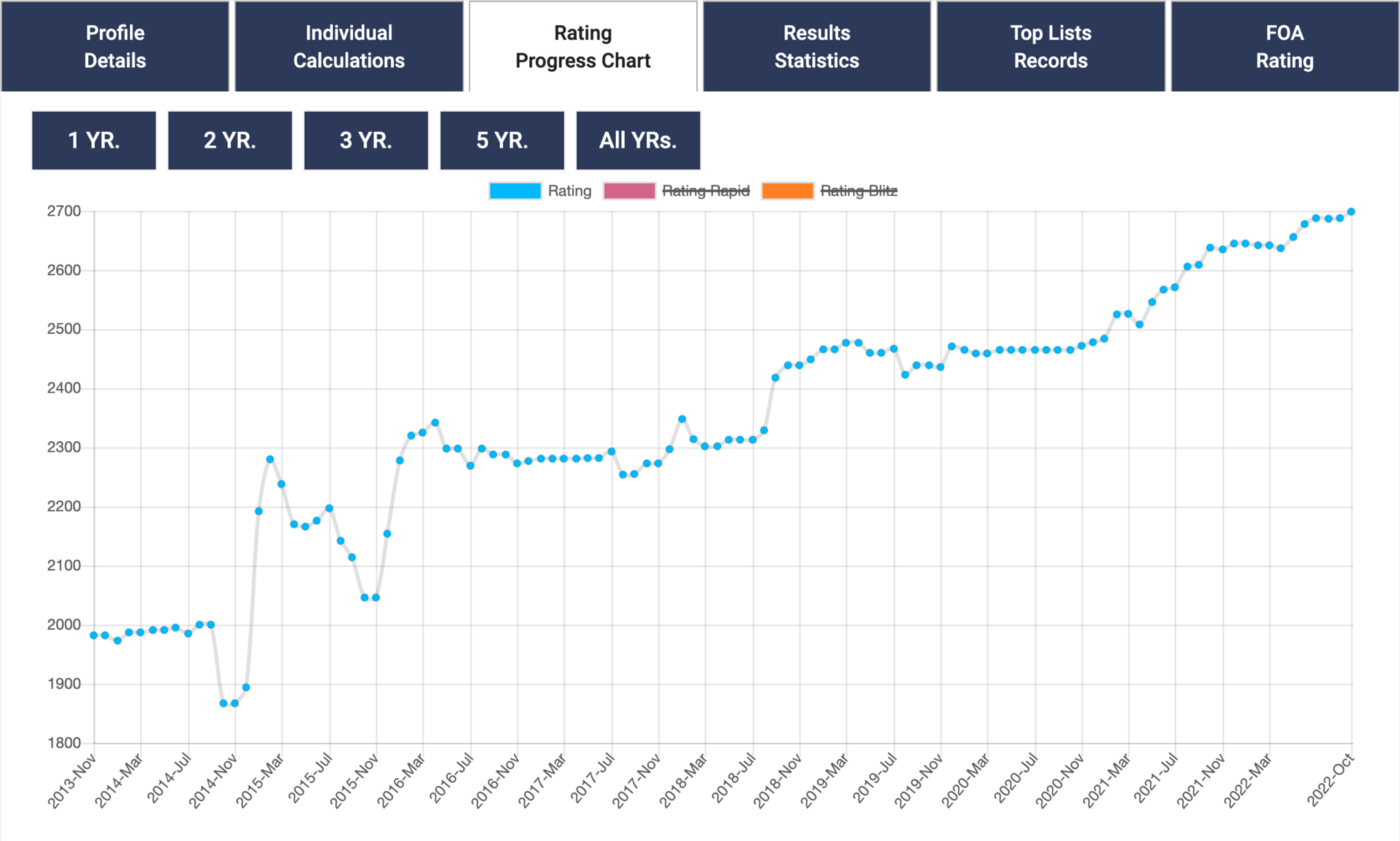
\includegraphics[scale=0.3]{niemann_rating.png}

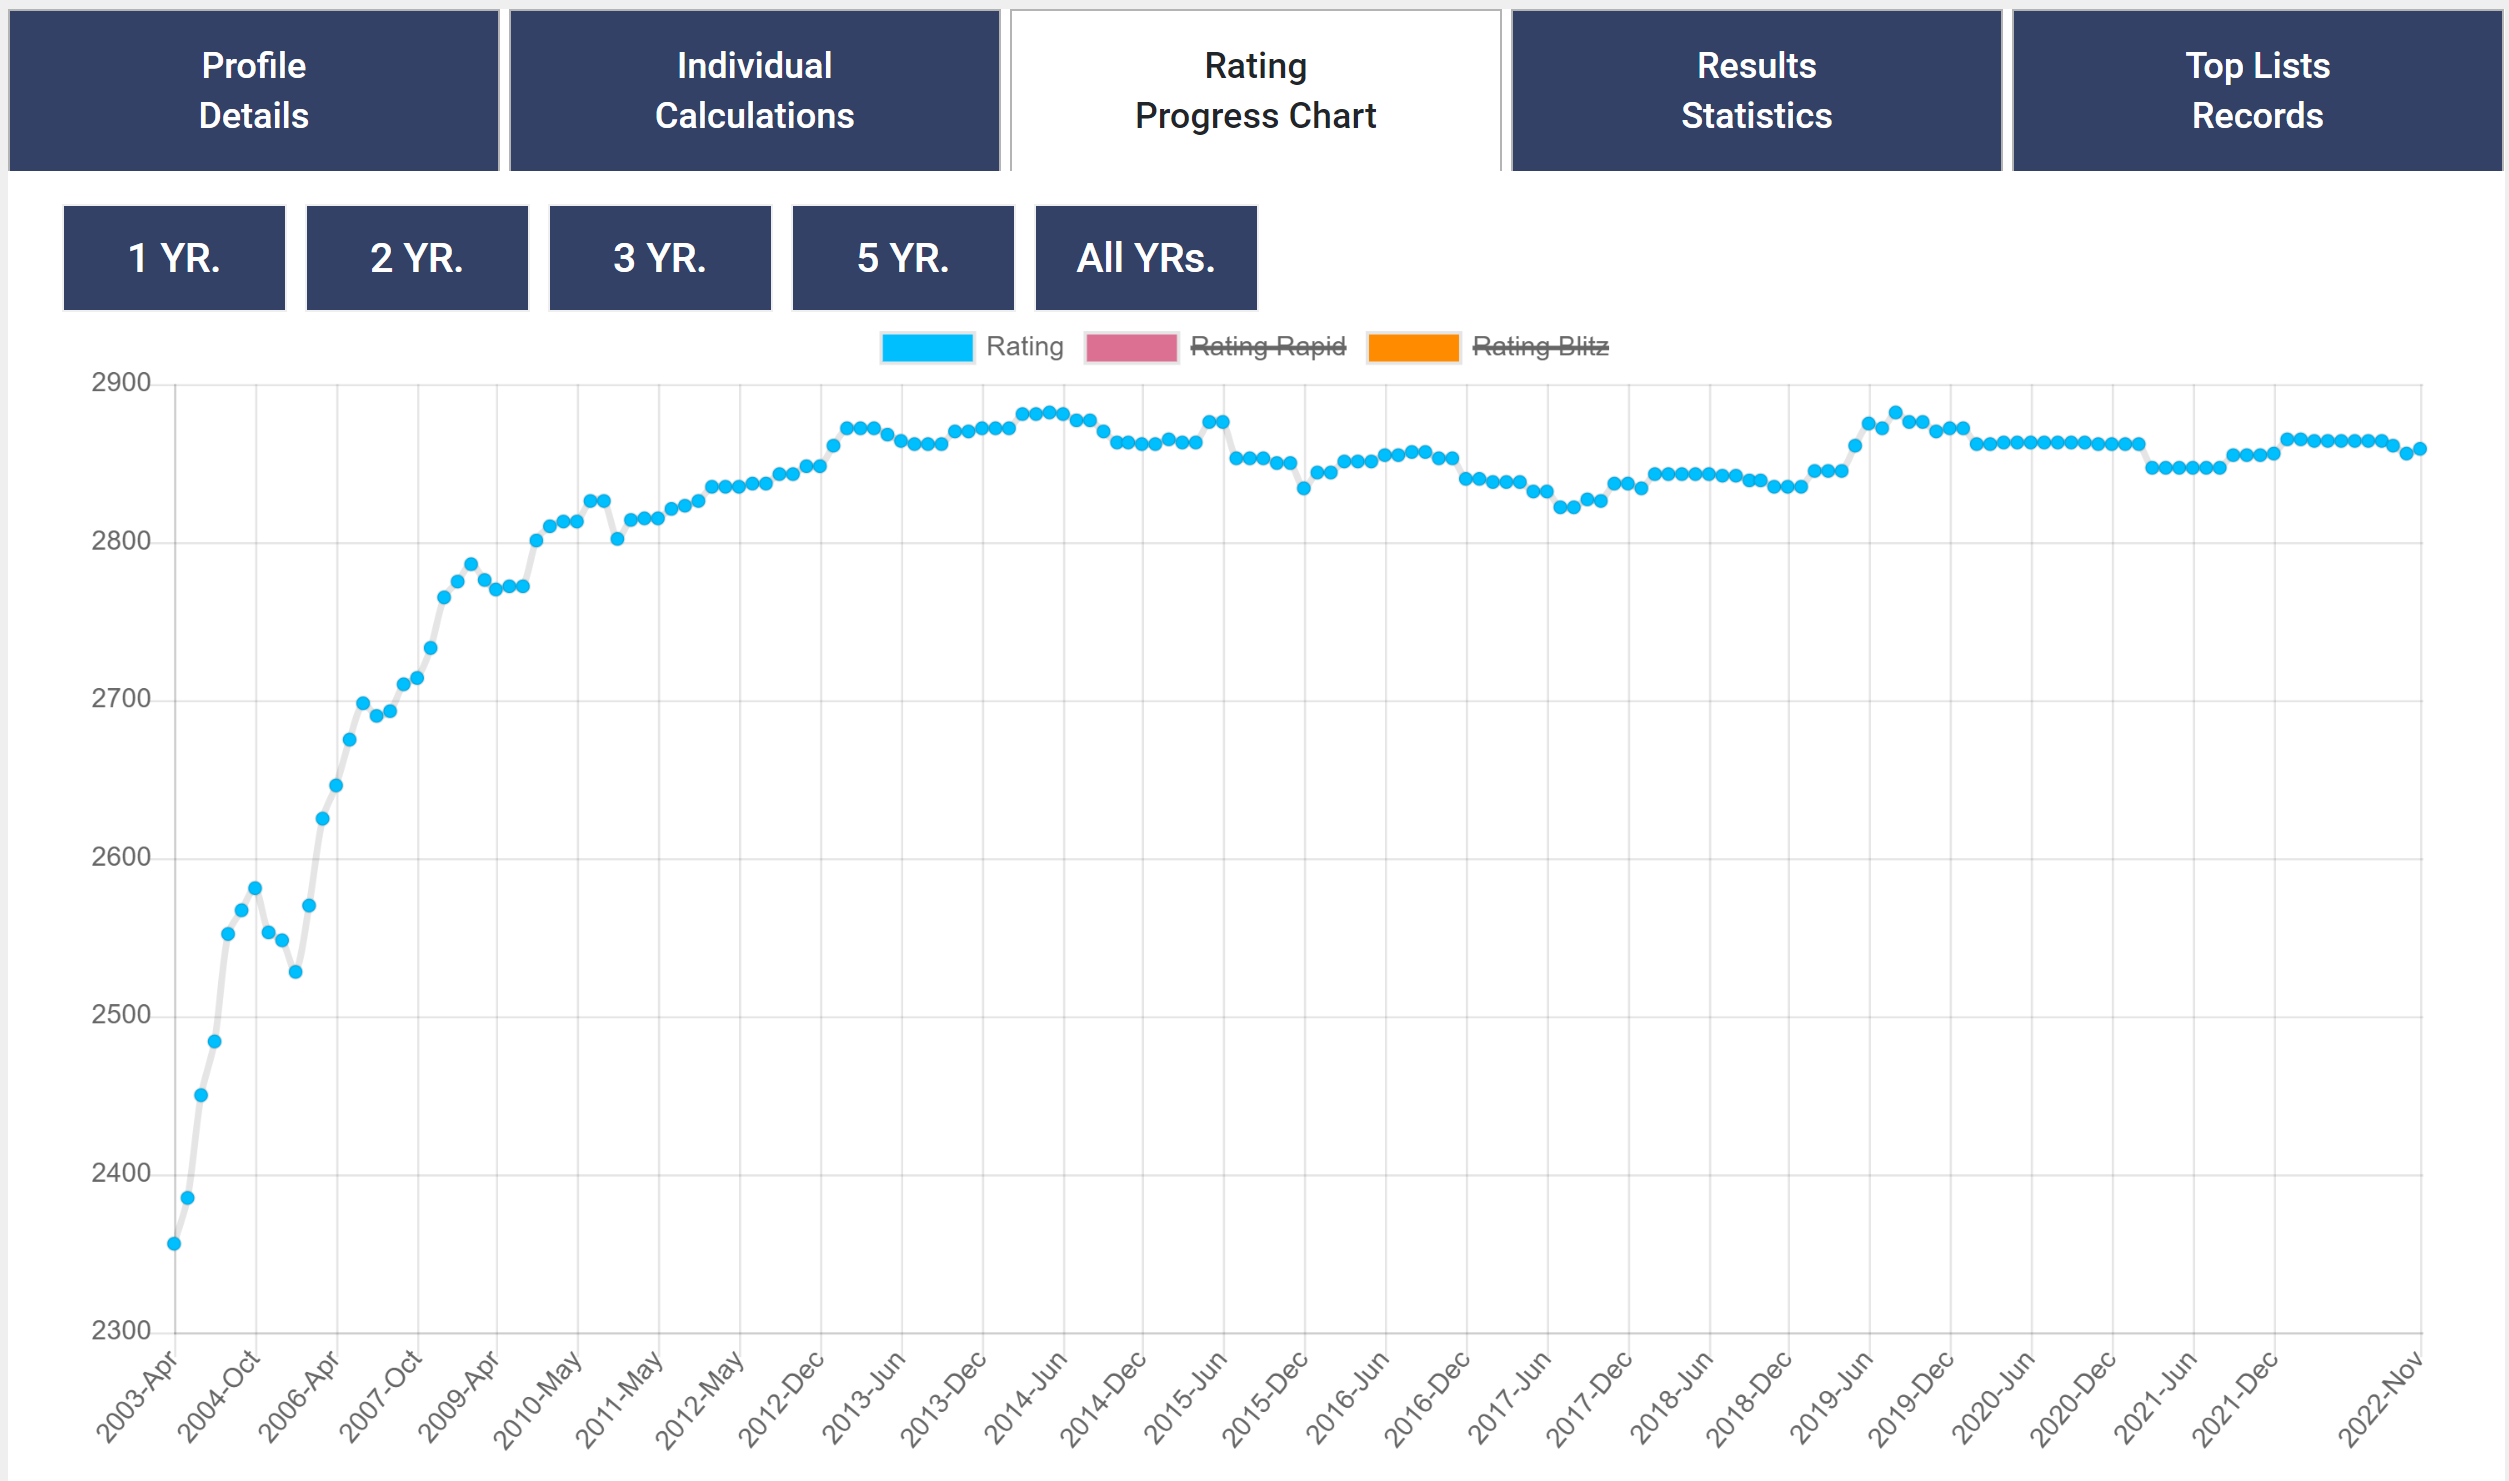
\includegraphics[scale=0.5]{carlsen_rating.png}

% report statistical analysis in tables/figures, summarize what they mean
% discussion to link analysis back to topic

\section*{Discussion}
\addcontentsline{toc}{section}{Discussion}
\label{sec:disc}

% summarize contributions of research and future directions
The results of this research largely confirm the claims included in Chess.com's report on Niemann however, although the data does indicate suspicious activity, this is not a "cut and dry" case of cheating, so to speak. Observing a single method to detect cheating as we have through average centipawn loss is not enough to confirm for sure that Hans Niemann cheated, both virtually and OTB, more than he claimed but this was never truely the objective of this research. The real question posed here was whether historical records of average centipawn loss compared to his ELO ranking could be treated as a "smoking gun" or surefire way to prove cheating alone; which it does not. Note: Relevant figures not available, fix this later. 

\section*{Appendix}
\addcontentsline{toc}{section}{Appendix}
\label{sec:appx}

\section*{References}
\addcontentsline{toc}{section}{References}
\label{sec:refs}

\end{document}